\documentclass[10pt,a4paper]{article}
\usepackage[utf8]{inputenc}

% Define the page margin
\usepackage[margin=3cm]{geometry}

% Better typography (font rendering)
\usepackage{microtype}

% Math environments and macros
\usepackage{amsmath}
\usepackage{amsfonts}
\usepackage{amssymb}
\usepackage{amsthm}

% Define \includegraphics to include graphics
\usepackage{graphicx}

% Draw graphics from a text description
\usepackage{tikz}

% Syntax highlighting
\usepackage{minted}

% Set global minted options
\setminted{linenos, autogobble, frame=lines, framesep=2mm}

% Import the comment environment for orgtbl-mode
\usepackage{comment}

% Do not indent paragraphs
\usepackage{parskip}

\title{Operating Systems, Sheet 5}
\author{Marten Lienen (03670270)}

\begin{document}

\maketitle

\section*{Exercise 1}

\subsection*{Part 1.1)}

(1) ist sinnvoll, weil die Summe der belegten plus der noch unbelegten Resourcen die Gesamtanzahl der verfügbaren Resourcen sein sollten.
(2) ist sinnvoll, weil kein einzelner Prozess mehr von einer Resourcen belegen/anfordern können sollte als insgesamt existiert.

\subsection*{Part 1.2)}

\subsubsection*{Szenario 1}

Die Anforderung von 3 kann erfüllt werden.
Wenn dann 3 alles freigibt, kann danach 4 oder 2 die Resourcen zugeteilt bekommen.
Danach kriegt der jeweils andere Prozess den Zugriff.
Zuletzt ist dann genug Kapazität vorhanden, um Prozess 1 ohne Probleme Zugriff zu erteilen.

\subsubsection*{Szenario 2}

Solange niemand freigibt, kann keine Anforderung erfüllt werden und das System befindet sich in einem Deadlock.

\subsubsection*{Szenario 3}

Das System befindet sich ebenfalls in einem Deadlock, weil die Anforderung keines Prozesses erfüllt werden können, indem ihm nur mehr von Resource 1 oder 3 zugeteilt wird.

\subsection*{Part 1.3)}

Weil einem Betriebssystem nicht bekannt ist, wieviel von welcher Resource ein Prozess bis zur Freigabe der belegten Resourcen noch anfordern wird.

\section*{Exercise 2}

\subsection*{Part 2.1)}

Diese Lösung ist ein bisschen simplifiziert, aber sollte alle wichtigen Dinge abdecken.
Weggelassen habe ich, dass der Mitarbeiter bzw. die Lastwagen immer erst beladen werden, also jeweils eine Stelle für diese, und weitere Transitionen um Betten und Schränke zu verkaufen.

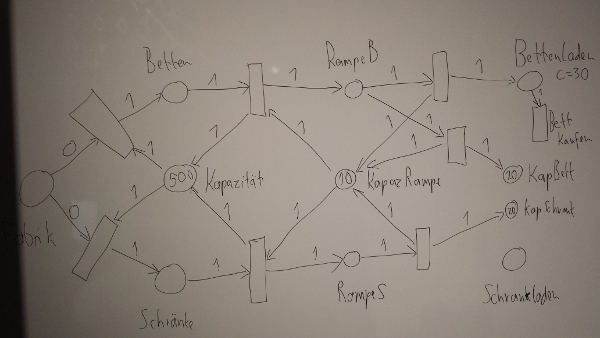
\includegraphics[width=\textwidth]{sheet-5/exercise-2}

\section*{Exercise 3}

\inputminted{c}{sheet-5/main.c}

\end{document}
